\section{Autoencoders}

\begin{frame}{Pardon the Interruption \dots}

TODO reviewer comment

\end{frame}

\begin{frame}{Autoencoder Intuition}

two superpowers of autoencoders:
\begin{itemize}

\item compression (bottlenecked autoencoder)

\item de-corruption (denoising autoencoder)

\end{itemize}

\end{frame}

\begin{frame}{Autoencoder Intuition: Bottlenecked}

TODO Police Artist 1

\end{frame}

\begin{frame}{Autoencoder Intuition: Bottlenecked}

Why does this work?

\begin{itemize}

\item faces are a \textit{subset} of all possible images
\item detective and witness have seen lots of faces, learned how to describe face

\end{itemize}

\end{frame}

\begin{frame}{Autoencoder Example: Bottlenecked}

face montage

\end{frame}

\begin{frame}{Autoencoder Example: Bottlenecked}

what is a latent-space interpolation?

\end{frame}

\begin{frame}{Autoencoder Intuition: Denoiser}

TODO Police Artist 2

\end{frame}

\begin{frame}{Autoencoder Intuition: Denoiser}

Why does this work?

\begin{itemize}

\item faces are a \textit{subset} of all possible images
\item symmetries, correlations, and certain universal characteristics of faces $\rightarrow$ fix incomplete/corrupted input
\begin{itemize}
\item usually, eye color is same left/right
\item blue eyes correlated with blond hair
\item faces have same general eye-nose-mouth layout
\end{itemize}

\end{itemize}

\end{frame}

\begin{frame}{Autoencoder Intuition: Example}

face reconstruction

\end{frame}

\begin{frame}{Autoencoder Implementation}

How exactly does this all work?

deep learning

(a.k.a. big artificial neural networks tuned with lots of training data)

\end{frame}

\begin{frame}{Autoencoder Implementation}

\begin{figure}
        \begin{subfigure}[b]{0.50\textwidth}
          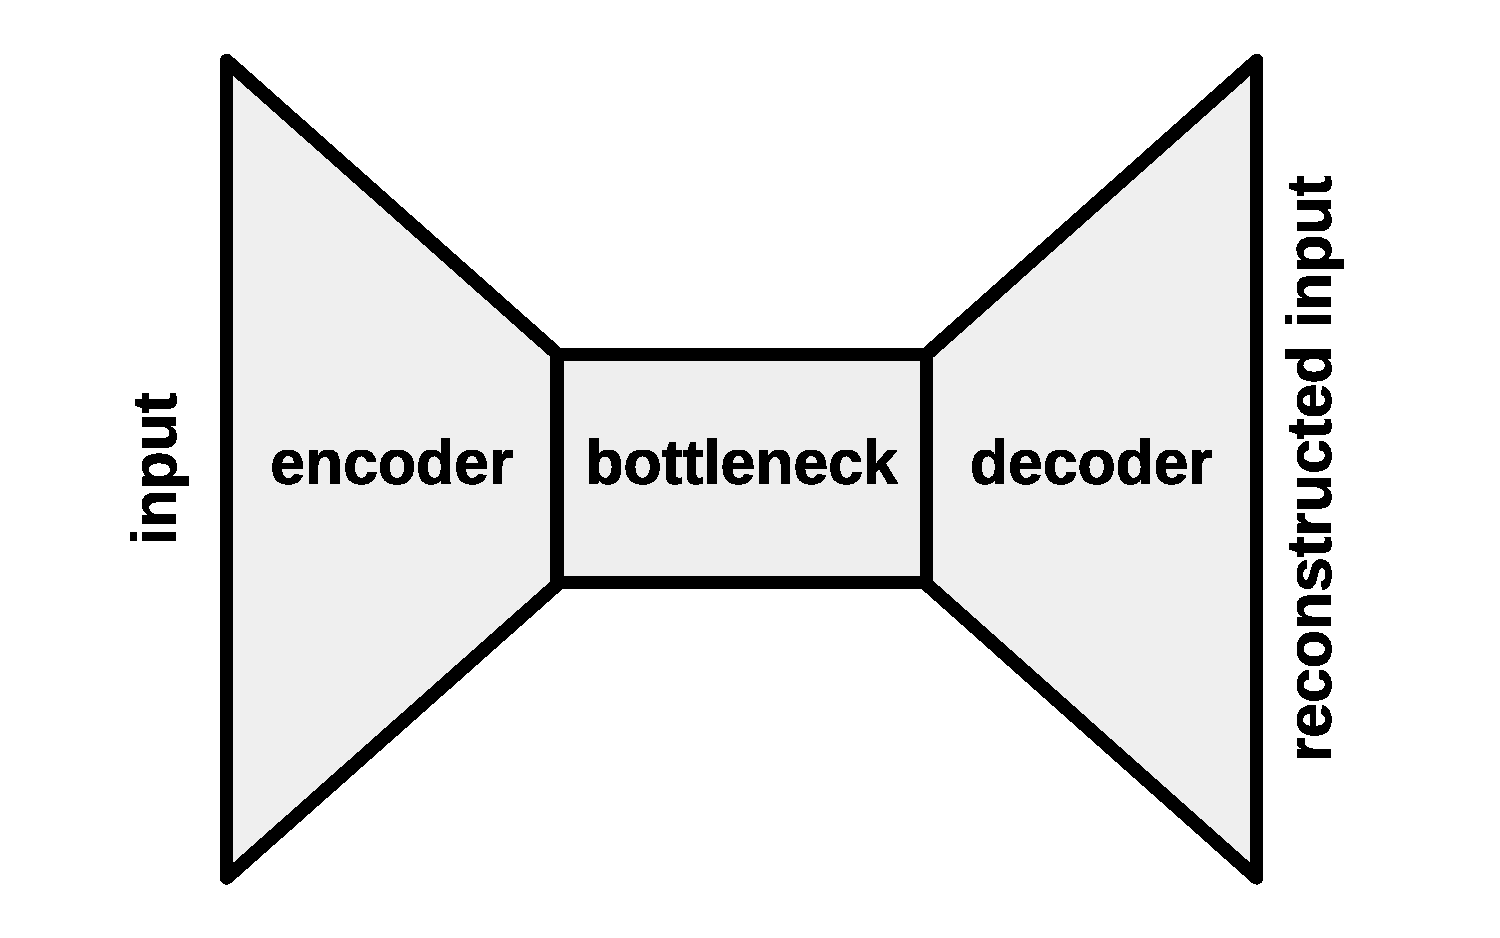
\includegraphics[width=\textwidth]{img/bottleneck}
          \subcaption{bottleneck autoencoder}
          \label{fig:bottleneck}
        \end{subfigure}%
        \begin{subfigure}[b]{0.50\textwidth}
          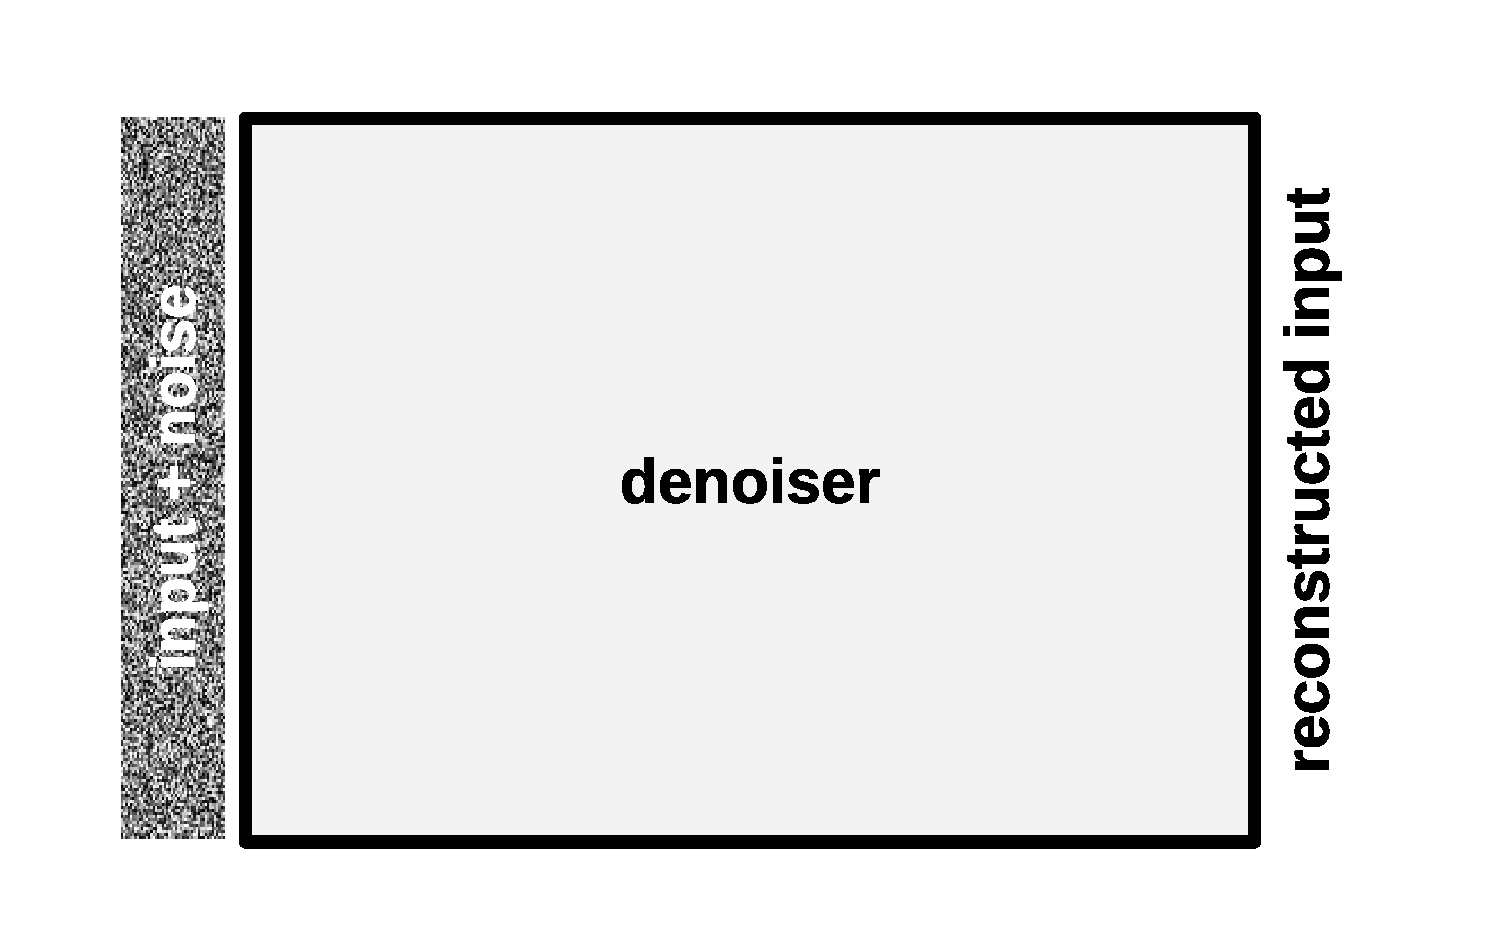
\includegraphics[width=\textwidth]{img/denoiser}
          \subcaption{denoising autoencoder}
          \label{fig:denoiser}
        \end{subfigure}%
        \caption{
          Schematics of bottlenecked a denoising autoencoders.
        }\label{fig:autoencoders}
\end{figure}


\end{frame}
